\documentclass[12pt]{article}
\usepackage[a4paper,
            inner=10mm,
            outer=50mm, % = marginparsep + marginparwidth 
                       %   + 5mm (between marginpar and page border)
            top=20mm,
            bottom=25mm,
            marginparsep=5mm,
            marginparwidth=40mm,
            % showframe
            ]{geometry}
\usepackage{amsfonts}
\usepackage{amsmath}
\usepackage{xcolor}
\usepackage{todonotes}
\usepackage{pythonhighlight}

% define command for grey colored text
% \newcommand{\note}[1]{ \textit{\textcolor{gray}{... #1 ...}} }
\newcommand{\note}[1]{\todo[color=yellow!40,bordercolor=none,linecolor=black]{#1}}
\tolerance=1
\emergencystretch=\maxdimen
\hyphenpenalty=10000
\hbadness=10000

% bibilography management
\usepackage[style=numeric]{biblatex}
\addbibresource{bibs.bib}

\begin{document}

\listoftodos

\tableofcontents

\section{Introduction}

\note{8 - 10 pages of introduction}

\textbf{Deep Learning (DL)} is a branch of \textbf{Artificial Intelligence (AI)} that emphasizes the use of neural networks to fit the inputs and outputs of a dataset.
The training of a neural network is done by computing the gradients of the loss function with respect to the weights and biases of the network.
A better trained neural network can better approximate the function that maps the inputs to the outputs of the dataset.

\textbf{Reinforcement Learning (RL)} is a branch of AI that emphasizes on solving problems through trials and errors with delayed rewards.
RL had most success in the domain of \textbf{Game Playing}: making agents that could play boardgames, Atari games, or other types of games.
An extension to Game Playing is \textbf{General Game Playing (GGP)}, with the goal of designing agents that could play any type of game without having much prior knowledge of the games.
\note{discuss policy}

\textbf{Deep Reinforcement Learning (DRL)} is a rising branch that combines DL and RL techniques to solve problems.
In a DRL system, RL usually defines the backbone structure of the algorithm especially the Agent-Environment interface.
On the other hand, DL is responsible for approximating specific functions by using the generated data.

\textbf{Planning} refers to any computational process that analyzes a sequence of generated actions and their consequences in the enviornment.
In the RL notation, planning specifically means the use of a model to improve a policy.

A \textbf{Distributed System} is a computer system that uses multiple processes with various purposes to complete tasks.
% DRL systems 

\subsection{Contribution}
In this thesis we will describle a framework for solving the problem of GGP.
We first define a interaction interface that's similar to the Agent-Environment Interface established in the current literature.
We will also detail \textbf{MooZi}, a system that implements the GGP framework and the \textbf{MuZero} algorithm for playing both boardgames and Atari games.

\section{Literature Review}
\note{4 - 5 pages}

\subsection{Planning and Search}
\subsubsection{Introduction}
Most, if not all, AI problems can be reduced to a search problem \cite[p.39]{ArtificialIntelligenceGames_Yannakakis.Togelius_2018}.
Such search problems could be solved by determining the best plan, path, model, function, and so on, based some metrics of interest.
Therefore, search has been playing a vital role in AI research since its dawn.

The term \textbf{planning} and \textbf{search} are widely used across different domains, especially in AI, and sometimes interchangable.
Here we adopt the definition by \citeauthor{ReinforcementLearningIntroduction_Sutton.Barto_2018} \cite{ReinforcementLearningIntroduction_Sutton.Barto_2018}.

\textbf{Planning} refers to any process by which the agent updates the action selection policy $\pi(a \mid s)$ or the value function $v_\pi(s)$.
We will focus on the case of improving the policy in our discussion.
We could view the planning process as an operater $\mathcal{I}$ that takes the policy as input and outputs an improved policy $\mathcal{I}\pi$.

Planning methods could be categorized into types based on the focus of the target state $s$ to improve.
If the method improves the policy for arbitrary states, we call \textbf{background planning}.
That is, for any timestep $t$:
$$\pi(a \mid s) \leftarrow \mathcal{I}\pi(a \mid s), ~~ s \in \mathcal{S}$$
Typical background planning methods include dynamic programming and Dyna-Q.
In the case of dynamic programming, a full sweep of the state space is performed and all states are updated.
In the case of Dyna, an random subset of the state space is selected and all states in the subset are updated.

The other type of planning focuses on improving the policy of the current state $S_t$ instead of any state.
We call this \textbf{decision-time planning}.
That is, for any timestep $t$:
$$\pi(a \mid s) \leftarrow \mathcal{I}\pi(a \mid s), ~~ s = S_t$$

We could also use blend both types of planning together.
Technically, we could say that algorithms like AlphaGo use both types of planning when they self-play for training.
The decision-time part is straight-forward: a tree search is performed at the root node and updates the policy of the current state.
At the same time, the neural network is trained on past experience and all states are updated.
The updates of this background planning is applied when the planner pulls the latest weights of the neural networks.
% MooZi also implements MuZero Reanalyze, which means

% \note{describe search in general and with a focus on MCTS}

Early AI research has been focused on the use of search as a planning method.
In 1968, \citeauthor{FormalBasisHeuristic_Hart.Nilsson.ea_1968} designed the \textbf{A*} algorithm for finding shortest path from a start vertex to a target vertex \cite{FormalBasisHeuristic_Hart.Nilsson.ea_1968}.
Although A* works quite well for many problems, especially in early game AI, it falls short in cases where the assumptions of A* do not hold.
For example, A* does not yield optimal solution under stochastic environments and it could be computationally infeasible on problems with high branching factors.
More sophisticated search algorithms were developed to cater to the growing complexity of use cases.

In 1990, \citeauthor{RealtimeHeuristicSearch_Korf_1990} framed the problem of \textbf{Real-Time Heursitic Search},
proposed the Real-Time-A* algorith, and pioneered the study of search algorithms with bounded computation \cite{RealtimeHeuristicSearch_Korf_1990}.

Monte-Carlo techniques were adopted to handle environment stochasticity.
Tree-based search algorithms such as \textbf{MiniMax} and \textbf{Alpha-Beta Pruning} were also designed to better play two-player games.

\subsection{Monte Carlo Methods}
In 1873, Joseph Jagger observed the bias in roulette wheels at Monte Carlo Casino.
He studied the bias by recording results of roulette wheels and captialized over 2 million francs over several days by betting on the most favorably biased wheel \cite{MonteCarloCasino__2022}.
Therefore, \textbf{Monte Carlo (MC)} methods gained their name as a class of algorithms based on building expectation on random processes.

MC methods are used in many domains but in this thesis we will primarily focus on its usage in search.
In a game where terminal states are usually unreachable by the limited search depth, evaluations has to be performed on the leaf nodes that represent intermidate game states.
One way of obtaining an evaluation on a state is by applying a heursitic function.
Heursitic functions used this way are usually hand-crafted by human based on expert knowledge, and hence are prone to human error.
The other way of evaluating the state is to perform a rollout from that state to a terminal state by selecting actions randomly.
This evaluation process is called \textbf{random rollout} or \textbf{Monte-Carlo rollout}.

\subsection{Monte-Carlo Tree Search (MCTS)} \label{sec:MCTS}

\citeauthor{BanditBasedMonteCarlo_Kocsis.Szepesvari_2006} developed the \textbf{Upper Confidence Bounds applied to Trees (UCT)} method as an extension of the Upper Confidence Bound (UCB) employed in bandits \cite{BanditBasedMonteCarlo_Kocsis.Szepesvari_2006}.
Rémi Coulom developed the general idea of \textbf{Monte-Carlo Tree Search} that combines both Monte-Carlo rollouts and tree search \cite{EfficientSelectivityBackup_Coulom_2007} for Go program CrazyStone.
Shortly afterwards,
\citeauthor{ModificationUCTPatterns_Gelly.Wang.ea_2006} implemented MoGo that uses the UCT selection formula \cite{ModificationUCTPatterns_Gelly.Wang.ea_2006}.
MCTS is then generalized by \citeauthor{MonteCarloTreeSearch_Chaslot.Bakkes.ea_2008} as a framework for game AI \cite{MonteCarloTreeSearch_Chaslot.Bakkes.ea_2008}.
This framework requires less domain knowledge than other classic approaches to game AI while also being competent in strength.
% There are four steps in this framework that are iteratively applied to the search tree.
The core idea of this framework is to gradually build the search tree by iteratively applying four steps: \textbf{selction}, \textbf{expansion}, \textbf{evaluation}, and \textbf{backpropagation}.
The search tree built this way will have an emphasize on more promising moves and game states.
This means these more promising states are visited more often, have more children, and have deeper estimates that are aggregated to a more accurate value.

Here we detail the four steps in the MCTS framework by \citeauthor{MonteCarloTreeSearch_Chaslot.Bakkes.ea_2008} (see Figure \ref{fig:mcts}).

\begin{figure}[h]
    \centering
    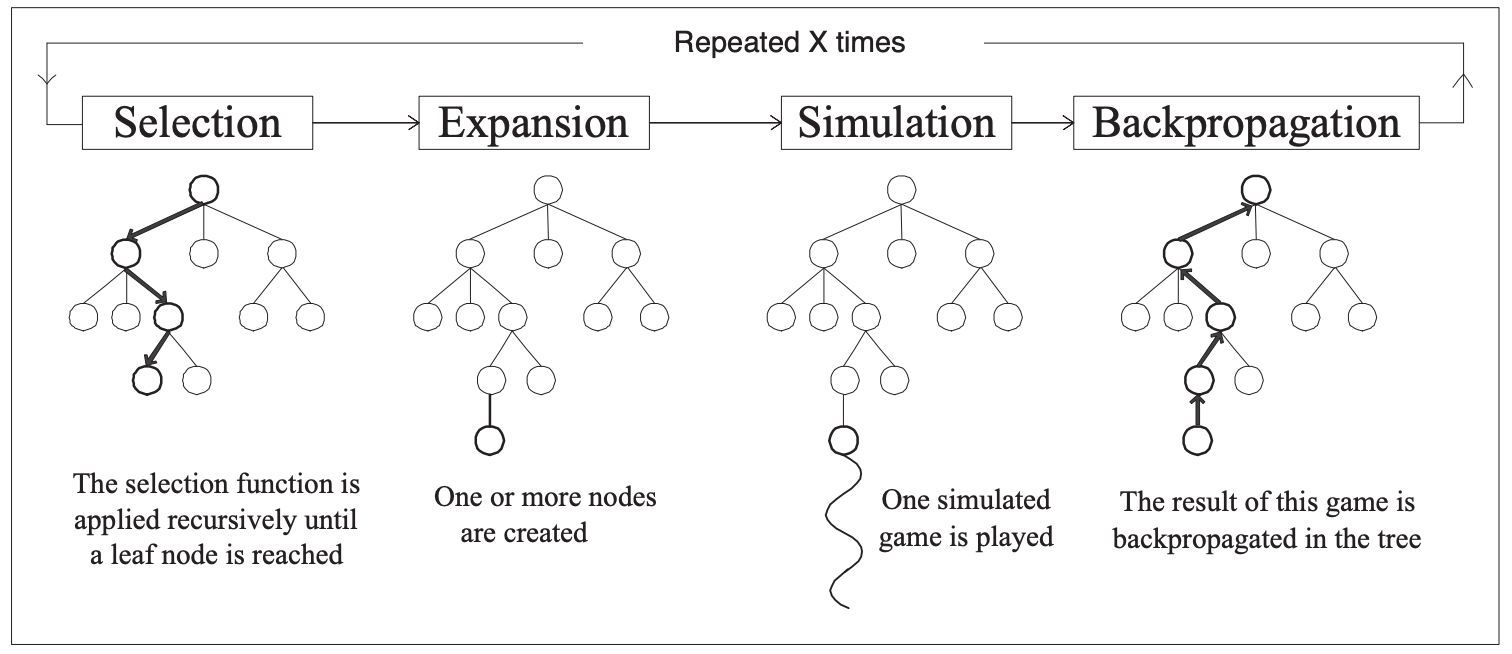
\includegraphics[scale=0.5]{assets/mcts.png}
    \caption[]{The Monte-Carlo Tree Search Framework}
    \label{fig:mcts}
\end{figure}

\subsubsection{Selection}
This selection process starts at the root node and repeats until a leaf node is reached.
At each level of the tree, a child node is selected based on a selection formula.
A selection formula usually has two parts, one part is based on the prior score $x$ of the state, and the other part is the exploration bonus $b$.
For a parent node $p$ and children nodes $C$, the selection $I$ is based on
\begin{equation}
    \label{eq:MCTS_selection}
    I_p = \operatorname{argmax}_{c \in C} \left( x_c + b_c \right)
\end{equation}

The prior score could be based on the value of the child, the accumulated reward of the child, or the prior selection probability based on the policy $\pi(c \mid p)$.
The exploration bonus is usually based on the visit count of the child and the parent.
The more visits a child gets, the less the exploration bonus will be.

For example, \citeauthor{ModificationUCTPatterns_Gelly.Wang.ea_2006} used this following formula for selection in their MoGo implentation:
$$
    I_p = \operatorname{argmax}_{c \in C} \left( \frac{v_c}{n_c} + \sqrt{\frac{2 * \log(n_b)}{n_c} } \right)
$$
where $v_c$ is the value of the node, $n_b$ and $n_c$ are the visit counts of the parent and child, respectively.

\subsubsection{Expansion}
The selected leaf node is then expanded by adding one or more children to the leaf node, each represents a succeeding game state of the selected leaf's state.

\subsubsection{Evaluation}
Each of the expanded nodes is now evaluated by using one of these methods:
\begin{itemize}
    \item A game is played until the game ends using a random policy.
    \item A game is played until the game ends using a rollout policy.
    \item A evaluation function is applied to the node.
          This evaluation function could be either a hand-crafted heursitic
          or learned by a neural network
\end{itemize}

\subsubsection{Backpropagation}
After the expanded nodes are evaluated, the traversed nodes to reach the expanded nodes are updated.
The statistics updated usually include visit count, estimated value and accumulated reward of the nodes.

These four steps are repeated until the budget runs out.
After this search is performed, the agent acts by selecting the action associated with the most promising child of the root node.
This could be the most visited child, the child with the greatest value, or the child with the highest lower bound.

\subsection{AlphaGo, AlphaGo Zero, and Alpha Zero}
\textbf{AlphaGo} is the first Go program that beats a human Go champion by 5 games to 0.
% AlphaGo learns a policy net that maps states to actions, and a value net that maps states to values.
The AlphaGo is trained with a machine learning pipeline with multiple stages.
For the first stage of training, a supervised learning policy (or SL policy) is trained to predict expert moves.
This SL policy $p$ is parametrized by weights $\sigma$, denoted $p_{\sigma}$.
The input of the policy network is a representation of the board state, denoted $s$.
Given a state $s$ as the input, this network outputs a probability distribution over all legal moves $a$ through the last softmax layer.
During the training of the network, randomly sampled expert moves are used as training targets.
The weights $\sigma$ are then updated through gradient ascend to maximize the probability of matching the human expert move:
$$
    \Delta \sigma \propto \frac{\partial \log p_{\sigma}(a \mid s)}{\partial \sigma}
$$
For the second stage of training, the supervised policy $p_{\sigma}$ is duplicated further trained with reinforcement learning.
This reinforcement learning trained policy (or RL policy) is parametrized by weights $\rho$ which is initialized to the same values as $\sigma$.
In other words, the RL policy is initialized so that $p_{\rho} = p_{\sigma}$.
The training data is then generated through self-play using $p_{\rho}$ as the rollout policy.
For each game, the game outcome $z_t = \pm r(s_T)$, where $s_T$ is the terminal state, $+1$ for winning, $-1$ for losing from the perspective of the current player.
Weights $\rho$ is then updated using gradient ascend to maximize the expected outcome using the update formula:
$$
    \Delta \rho \propto \frac{\partial \log p_{\rho}\left(a_{t} \mid s_{t}\right)}{\partial \rho} z_{t}
$$
For the last stage, a value function is trained to evaluate board positions.
This value function is modeled with a neural network with weights $\theta$, denoted $v_{\theta}$.
Given a state $s$, $v_{\theta}(s)$ predicts the outcome of the game as if both players act according to the policy $p_{\rho}$.
The neural network is trained with stochastic gradient descent to minimize the mean squared error (MSE) between the predicted value $v_{\theta}(s)$ and the outcome $z$.
$$
    \Delta \theta \propto \frac{\partial v_{\theta}(s)}{\partial \theta}\left(z-v_{\theta}(s)\right)
$$

AlphaGo combines the policy network $p_{\rho}$ and the value network $v_{\theta}$ with MCTS for acting.
AlphaGo uses a MCTS variant similar to that described in \ref{sec:MCTS}.
In the search tree, each edge $(s, a)$ stores an action value $Q(s, a)$ a visit count $N(s, a)$, and a prior probability $P(s, a)$.
At each time step, the search starts at the root node and simulates until the budget runs out.
In the select phase of each simulation phase, an action is selected for each traversed node using the same base formula (\ref{eq:MCTS_selection}).
In AlphaGo, the base score of the selection formula is the estimated value of the next states after taking the actions, namely $Q(s, a)$.
The exploration bonus of edge $(s, a)$ is based on the prior probability and decays as visit count grows.
\begin{equation}
    u(s, a) \propto \frac{P(s, a)}{1 + N(s, a)}
\end{equation}

The action taken at time $t$ is the action that maximizes the sum of the base score and the exploration bonus
\begin{equation}
    a_{t}=\underset{a}{\operatorname{argmax}}\left(Q\left(s_{t}, a\right)+u\left(s_{t}, a\right)\right)
\end{equation}

% \begin{itemize}
%     \item An action value $Q(s, a)$.
%      When this edge is first explored, this value is initialized by takinig the action using a perfect model and evaluate the post-action state $s'$ with the value network $v_{\theta}(s')$.
%     \item  Initialized to 0 and incremented for each visit during the simulations.
%     \item Prior probability $P(s, a)$. Obtained by using the policy network $p_{\rho}(s)$.
% \end{itemize}


% More concretely, the update follows the REINFORCE formula developed by \citeauthor{SimpleStatisticalGradientfollowing_Williams_1992} \cite{SimpleStatisticalGradientfollowing_Williams_1992}.
% The policy net is first trained with 
% $$
% \Delta \sigma \propto \frac{\partial \log p_{\sigma}(a \mid s)}{\partial \sigma}
% $$

% AlphaGo generates the samples for training the policy net by immitating professional Go games.
% \note{four AlphaGo, Supervised learning of policy networksReinforcement learning of policy networksReinforcement learning of value networksSearching with policy and value networks}

\textbf{AlphaGo Zero} is a successor of AlphaGo with the main difference of not learning from human.

\textbf{Alpha Zero} reduces game specific knowledge of AlphaGo Zero so that the same algorithm could be also applied to Shogi and chess.

% \note{to be continued ...},

\subsection{MuZero}
\textbf{MuZero} is different from the Alpha Zero family where the model used for planning is learned instead of given.
This difference further reduces game specific knowledge required for the algorithm.
More specifically, MuZero no longer requires the access to a perfect model of the target game.
Instead, a neural network that learns from the game experience is used in the search to replace the perfect model.

Central to MuZero's design are three functions trained for acting and planing.
The \textbf{representation function} $h$ encodes a history of observations $o_1, o_2, ..., o_t$ into a hidden state $s_t$.
The \textbf{dynamics function} $g$, given a hidden state $s^k$ and action $a^k$, produces an immediate reward $r^k$ and the next hidden state $s^{k+1}$.
The \textbf{prediction function} $f$, given a hidden state $s^k$, produces a probability distribution $p^k$ of actions and a value associated to that hidden state $v^k$.

MuZero plans with a search method based on the MCTS framework (discussed in \ref{sec:MCTS}).
Due to the lack of access to a perfect model, MuZero's MCTS differs from a standard one in numerous ways.
The nodes are no longer perfect representations of the board states.
Instead, each node is associated with a hidden state $s$ as a learned representation of the board state.
The transition is no longer made by the perfect model but the dynamics function.
There are technically no terminal states in the tree as the learned model does not predict game termination.
For timestep $t$, the search starts by creating the root node of the search tree with a history of observations
using the representation function
\begin{equation*}
    s^0 \leftarrow h_{\theta}(o_0, o_1, o_2, ..., o_t)
\end{equation*}
Then an action is selected base on

% These three functions are trained jointly 

% dynamics, and prediction functions.

% The representation function h outputs the initial hidden state s0, which is the root of the search tree by receiving history of the board for classic games and recent frames of the game concatenated by recent actions for Atari games. Dynamics function g produces the next hidden state sk and an immediate reward rk by getting previous hidden state sk−1 and a candidate action ak. Last but not least, the value vk and the policy to play pk for hidden state sk is defined by prediction function f.


% To act in the environment, At each timestep t, the presentation function generates an initial hidden state s0 as the root of Monte-Carlo Tree Search. Thereafter, by using prediction function’s outputs as priors and dynamics function to generate new hidden states and intermediate rewards within the tree, 800 simulations for board games and 50 simulations for Atari games are executed. The search policy finally specifies the next action at+1, by which the environment generates a new observation ot+1 and reward ut+1. At the end of the episode, the trajectory data is stored into a replay buffer to be used in the training process.
% During training, the MuZero network is unrolled for K (is considered 5) hypothetical steps and aligned to sequences sampled from the trajectories generated by the MCTS actors. Sequences are selected by sampling a state from any game in the replay buffer, then unrolling for K steps from that state. The parameters of all three functions are jointly trained, end-to-end by backpropagation-through-time. The policy, value function, and reward are improved by search probabilities pk ≈ πt+k, sample returns vk ≈ zt+k, and immediate rewards rt+k ≈ ut+k, respectively. The sample returns z could be final reward (board games) or n-step return (Atari games).


\section{Problem Definition}
\note{(5 pages)}

\subsection{Agent-Environment Interface and Markov Decision Process}
Traditionally, RL problems and solutions are frame with the \textbf{Agent-Environment Interface} (Figure \ref{fig:agent_environment_interface}).

\begin{figure}[h]
    \centering
    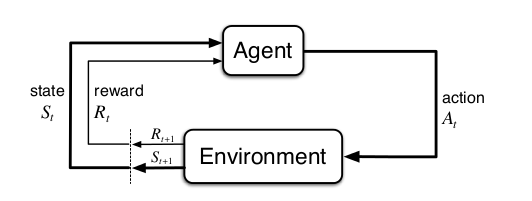
\includegraphics[scale=0.5]{assets/agent_environment_interface.png}
    \caption[]{Agent-Environment Interface}
    \label{fig:agent_environment_interface}
\end{figure}

The decision maker in this interface is called the \textbf{Agent}, and the agent interacts with the \textbf{Environment} continuously.
A problem implements the interface could be represented as a \textbf{Markov Decision Process (MDP)}, which is tuple of four elements where:
\begin{itemize}
    \item $\mathcal{S}$, a set of states that forms the \textit{state space}
    \item $\mathcal{A}$, a set of actions that forms the \textit{action space}
    \item $P(s, a, s') = Pr[ S_{t+1} = s' \mid  S_t = s, A_t = a]$, the transition probability function
    \item $R(s, a, s')$ the reward function
\end{itemize}
At each time step $t$, the agent starts at state $S_t \in \mathcal{S}$, picks an action $A_t \in \mathcal{A}$
transitions to state $S_{t+1} \in \mathcal{S}$ based on the probability function$P(S_{t+1} \mid S_t, A_t)$,
and receives a reward $R(S_t, A_t, S_{t+1})$.

The agent interacts with enviornment and generates a sequence of actions, states, and rewards:
$S_{0}, A_{0}, R_{1}, S_{1}, A_{1}, R_{2}, \dots$
We call this sequence a \textbf{trajectory}.
In the finite case, this interaction terminates until a terminal state is reached at time $t = T$, and this sequence is called an \textbf{episode}.
In the infinite case, the interaction continues indefinitely.
The goal of the agent in the problem is either to maximize the accumulative reward in the finite setting,
or to maximize the average reward in the infinite case.

\note{also describes policy $\pi$}

\note{address this is the most common formulation and how different libraries implement the interface}

\subsection{Shortcomings of the Agent-Environment Interface for General Game Playing}
% \note{I'm not sure if I should address these separatly.}
\subsubsection{Multi-Agent Games}
\note{address OpenSpiel's design multiple agents}
\subsubsection{Partial Observability}
\note{address POMDP}
\subsubsection{Environment Stochasticity}
\note{address OpenSpiel's design of random node}
\subsubsection{Episodic vs Continuous}
\note{barely seen in the literature, need more literature review}
\subsubsection{Self-Observability}
% \note{agent needs to be able to observe itself}
\subsubsection{Environment Output Structure}
% The agent-environment interface specifies two return types from the environment, namely the \textbf{observation} and the \textbf{reward}.
% All environment implementations used in the RL field follow 

\subsection{Our Approach}
\note{(5 pages)}

% The most significant difference of our approach is the separation of data and process.
% In the Agent-Environment Interface, both the agent and the environment are assumed to be stateful, which means they could store and process arbitrary data.

\subsubsection{Generalized Interaction Interface}
We propose the \textbf{Generalized Interaction Interface (GII)}.
We define the \textbf{tape} $E$ as the data storage of the interface, and a \textbf{law} $L$ as a pure function that operates on the tape.
An instance of such interface could consists of exactly one tape and multiple laws, and we define such an instance a \textbf{universe}.
A universe \textbf{ticks} by applying the laws on the tape.
\note{elaborate formally}

We implement a simplified version of this interface in \textbf{MooZi}.

% \note{elaborate on the interface}

\subsubsection{Advantages}
\note{pure functions are efficient}

\section{Method}
\note{(20 - 25 pages)}
\subsection{Design Philosophy}

\subsubsection{Use of Generalized Interaction Interface}
One of the goals of the project is to demostrate the use of Generalized Interaction Interface (GII).
All modules in the project will be implemented to align with the interface.
Third-party libraries that include game environments are wrapped with special wrappers that converts the outputs into the GII format.

\subsubsection{Use of Pure Functions}
One of the most notable difference of MooZi implementation is the use of pure functions.
In GII, \textbf{laws} are pure functions that read from and write to the \textbf{tape}.
Agents implemented in Agent-Environment Interface usually do not separate the storage of data and the handling of data.
In MooZi, we separate the storage of data and the handling of data whenever possible, especially for the parts with heavy compuations.
For example, we use \textbf{JAX} and \textbf{Haiku} to implement neural network related modules.
These libraries separate the \textbf{specification} and the \textbf{state} of a neural network.
The \textbf{specification} of a neural network is a pure function that is internally represented by a fixed computation graph.
The \textbf{parameters} of a neural network includes all variables that could be used with the specification to perform a forward pass.
\note{add one or two more examples of using pure functions, also mention how tape in the MooZi is different from the tape in GII}

\subsubsection{Being User Friendly}


\subsubsection{Training Efficiency}
One common problem with current open-sourced MuZero projects is their training efficiency.
Even for simple environments, these projects could take hours to train.
\note{
    Data needed; I've seen multiple issues on GitHub complaining about the training speed.
    I once assigned the task of "actually running the project and gather run time data" to Jiuqi but no follow up yet.
}

There are a few major bottlenecks of training efficiency in this type of project.
The first one is system parallelization.
\note{include data from previous presentation to make the point}

The second one is the environment transition speed.
\note{boardgames are fine, Atari games are slow, but in either cases we can't control}
% Board games, especially those are implemented in \textbf{OpenSpiel}, are faster.

The third one is neural network inferences used in training.
\note{MCTS inference batching is slow due to IO overhead, include data here from previous presentation to make the point}

% According to our deGeneralized Interaction Interface
\subsection{Structure Overview}

\begin{figure}[h]
    \centering
    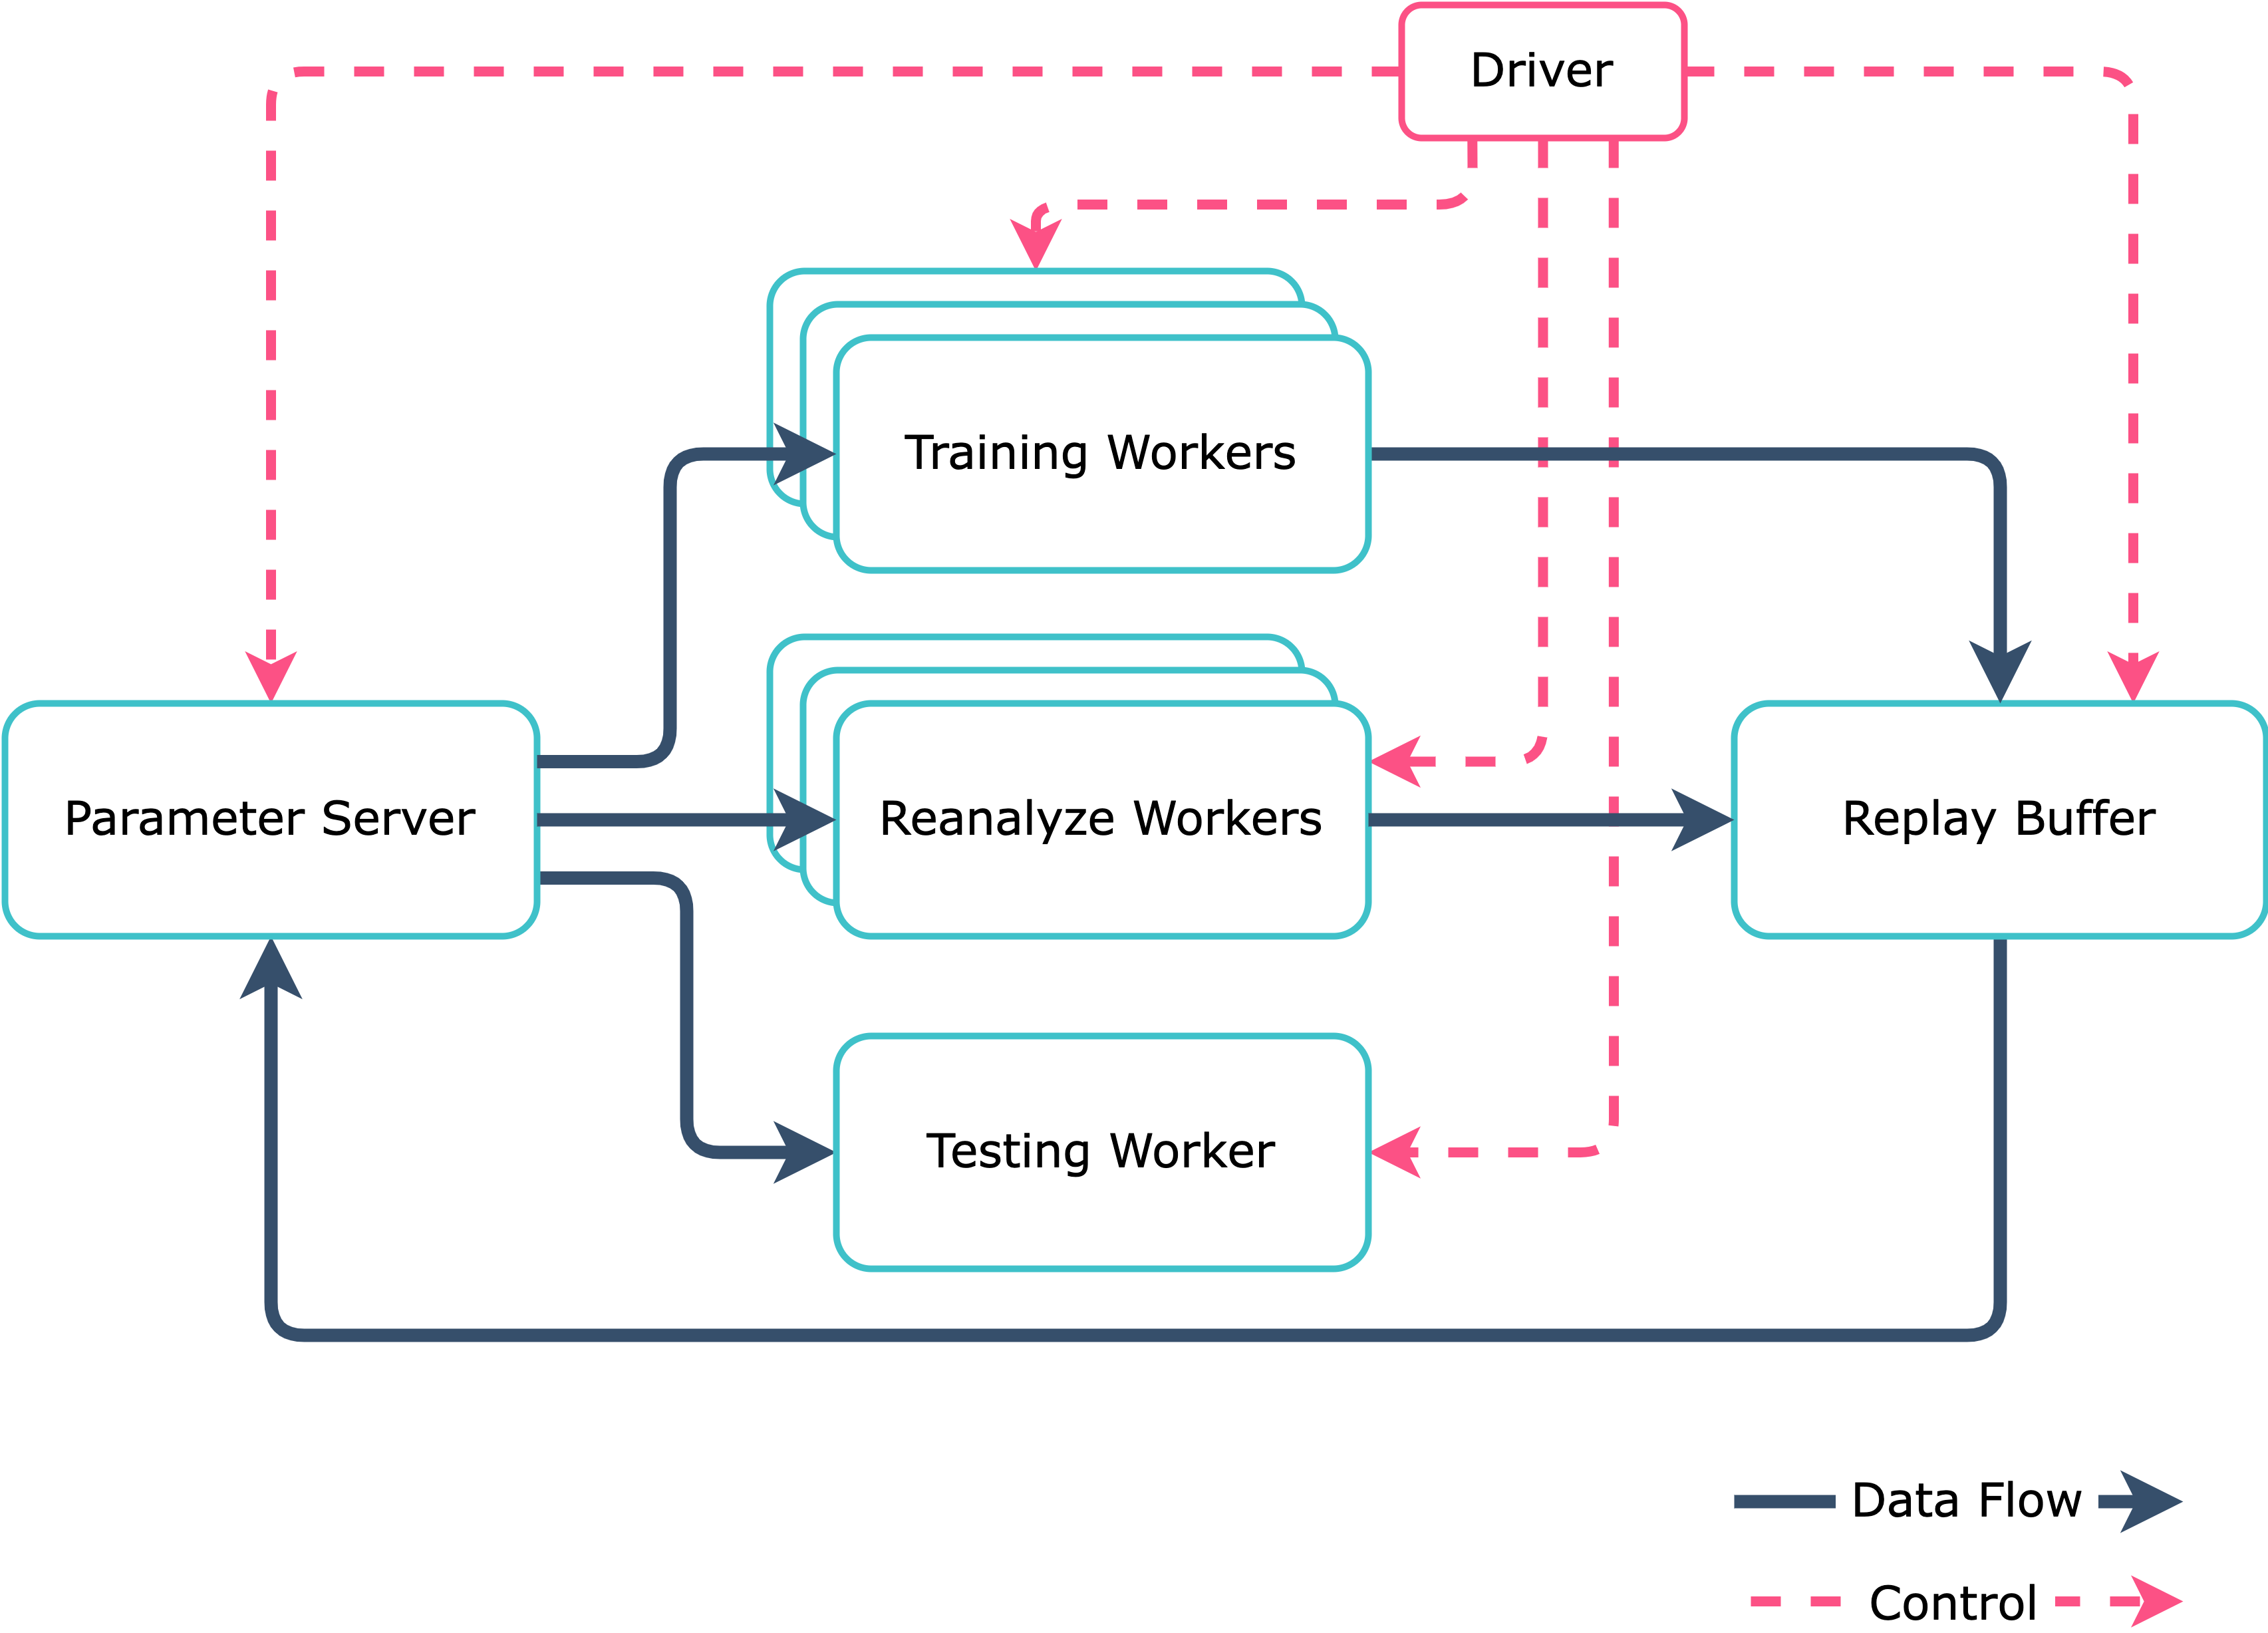
\includegraphics[width=\textwidth]{assets/moozi_architecture.png}
    \caption[]{MooZi Architecture}
    \label{fig:moozi_architecture}
\end{figure}

\subsubsection{Driver}
% MooZi adopts the \textbf{centralized control} design paradigm.
In a distributed system with centralized control, a single process is responsible for operating all other processes.
This central process is called the \textbf{driver}.
Other processes are either \textbf{tasks} or \textbf{actors}.
\textbf{Tasks} are stateless functions that takes inputs and return outputs.
\textbf{Actors} are statefull objects that group several methods that take inputs and return outputs.
In RL literature, \textbf{actor} is also a commonly used term to describe the process that stores a policy and interacts with an environment.
Even though MooZi does not adopt the concept of a RL actor, we will use the term \textbf{ray task} and \textbf{ray actor} to avoid confusion.
In contrast to distributed systems with distributed control, ray tasks and ray actors are reactive and do not have busy loops.
The driver decides when a ray task or ray actor is activated and what data should be used as inputs and where the outputs should go.
In other words, the driver process orchestrates the data and control flow of the entire system, and ray tasks and ray actors merely response to instructions.

\subsubsection{Environment Adaptors}
Environment adaptors unify environments defined in different libraries into a unified interface.
In the software engineering nomenclature, environment adaptors follow the adaptor design pattern \cite{AdapterPattern__2022}.

More specifically, in our project we implement environment adaptors for three types of environments that are commonly used in RL research:
(1) OpenAI Gym (2) OpenSpiel (3) MinAtar.
The adaptors convert the inputs and outputs of these environments into forms that GII accepts.

% Let's compare the libraries mentioned above with the agent-enviornment interface.
% In the agent-environment interface, the input to the enviornment is always a single action.
% Some of OpenSpiel's environments 

% return dict(
%     obs=timestep.observation,
%     is_first=timestep.first(),
%     is_last=timestep.last(),
%     to_play=0,
%     reward=reward,
%     legal_actions_mask=legal_actions_mask,
% )

The adaptors have the same signature as follows:
\begin{itemize}
    \item Inputs
          \subitem \textbf{is\_first}: A boolean signals the episode start.
          \subitem \textbf{is\_last}: A boolean signals the episode end.
          \subitem \textbf{action}: An integer indiates the last action taken by the agent.
          The valid range of the action is $\left[0, \text{number\_of\_available\_actions}\right)$.
    \item Outputs
          \subitem \textbf{obs}:
          An N-dimensional array that represents the observation of the current timestep.
          \subitem \textbf{is\_first}: A boolean signals the episode start.
          \subitem \textbf{is\_last}: A boolean signals the episode end.
          \subitem \textbf{to\_play}: An integer indicates the next player to take a move.
          \subitem \textbf{reward}: A float indicates the reward of taking the given action.
          \subitem \textbf{legal\_actions\_mask}: A bit mask of legal action indicies.
\end{itemize}

\subsubsection{Rollout Workers}
A \textbf{rollout worker} is a ray actor that:
\begin{itemize}
    \item stores a collection of universes, including tapes and laws in the universes
    \item stores a copy of the neural network specification
    \item stores a copy of the neural network parameters
    \item optionally stores batching layers that enable efficient computation
\end{itemize}

A rollout worker does not inherently serve a specific purpose in the system and its behavior is mostly determined by the list of laws created with the universes.

There are three main patterns of rollout workers used in MooZi:
\textbf{interaction training rollout worker},
\textbf{interaction testing rollout worker},
and \textbf{reanalyze rollout worker}.

\subsubsection{Replay Buffer}
The replay buffer:
\begin{itemize}
    \item stores trajectories generated by the rollout workers
    \item processes the trajectories into training targets
    \item stores processed training targets
    \item computes and updates priorities of training targets
    \item responsible for sampling and fetching batches of training targets
\end{itemize}

\subsubsection{Parameter Optimizer}
The parameter optimizer:
\begin{itemize}
    \item stores a copy of the neural network specification
    \item stores the latest copy of neural network parameters
    \item stores the loss function
    \item stores the training state
    \item computes forward and backward passes and updates the parameters
\end{itemize}

\subsubsection{Distributed Training}

\begin{python}
    for epoch in range(num_epochs):
    for w in workers_env + workers_test + workers_reanalyze:
    w.set_params_and_state(param_opt.get_params_and_state())

    while traj_futures:
    traj, traj_futures = ray.wait(traj_futures)
    traj = traj[0]
    replay_buffer.add_trajs(traj)

    if epoch >= epoch_train_start:
    train_batch = replay_buffer.get_train_targets_batch(
    big_batch_size
    )
    param_opt.update(train_batch, batch_size)

    env_trajs = [w.run(num_ticks_per_epoch) for w in workers_env]
    reanalyze_trajs = [w.run() for w in workers_reanalyze]
    traj_futures = env_trajs + reanalyze_trajs

    if epoch % test_interval == 0:
    test_result = workers_test[0].run(120)

    for w in workers_reanalyze:
    reanalyze_input = replay_buffer.get_train_targets_batch(
    num_trajs_per_reanalyze_universe
    * num_universes_per_reanalyze_worker
    )
    w.set_inputs(reanalyze_input)

\end{python}

\note{explain driver pseudo-code}

\subsubsection{Monte-Carlo Tree Search}
%     - asynchronous
%     - batching layer

\subsubsection{Logging and Visualization}


\section{Experiments}
\note{(20 pages)}

\section{Conclusion}
\note{(3 pages)}
\subsection{Future Work}
\note{(1 page)}

\printbibliography

\end{document}

\subsection*{Artificial Intelligence}

% Artificial Intelligence (AI) is a branch of computer science that emphasizes the use of computer algorithms to solve problems likes humans.
To define the goals and methods of Artificial Intelligence (AI), we first need to define what is \textit{intelligence}.
Though there is no consensus on the exact definition of intelligence, here we adopt the definition by John McCarthy:
\begin{quote}
    Intelligence is the computational part of the ability to achieve goals in the world.
\end{quote}
The goal of AI is to develop computer algorithms that can solve problems and achieve goals in complex environments.
A diverse range of methods are designed as AI algorithms since the term has been coined.
\note{A simple list of AI algorithms, such as A*, symbolic}


\subsection*{Game Artificial Intelligence}
Perfect vs in-Perfect information
\subsection*{Planning}
lookahead search: A*, DFS, BFS

\subsection*{Distributed System for AI}
IMPALA, SEED
